%\chapter{Long Short-Term Memory}
\label{ch:lstm}

\index{lstm|(}

Some problems in Machine Learning, especially NLP-focused tasks, generally require some sort of \textbf{context} from previous iterations to form a more comprehensive understanding of the problem it is being given. 

When facing context-heavy sentences such, as, ``I am from Malta, and I speak \textit{Maltese}'', most models became unable to forge enough contextual clues\index{Contextual clues} in order to determine the nationality despite such clues, or \textbf{long-term dependencies}, being given earlier in the sentence \citep{bengio94}.

In order to solve this problem, \citet{hochreiter1997long} proposed the Long Short-Term Memory network, or LSTM. 

\section{LSTM Architecture}
This module is a type of Recurrent Neural Network (RNN), that is, a repeated chained module, with a gradient-based unit applied. The main difference is that the repeated module itself is different, with the LSTM module being composed of a series of gates named the \textbf{input gate}, \textbf{input gate},   described in Figure~\ref{fig:lstm_architecture}.

\begin{figure*}
	\centering
	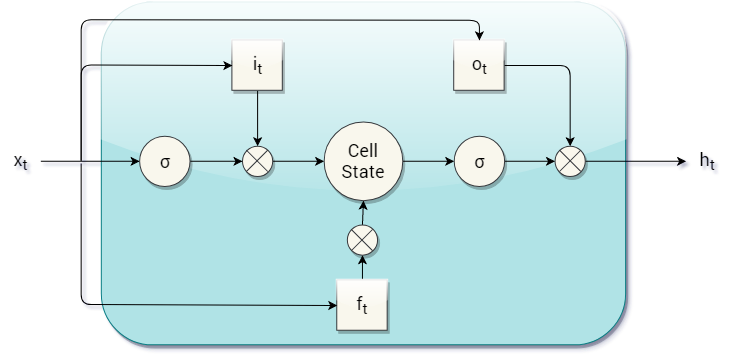
\includegraphics[width=0.6\linewidth]{graphics/lstm/lstm.png}
	\caption{
		Architecture of standard LSTM module.
	}
	\label{fig:lstm_architecture}
\end{figure*}

The traversal from one gate to another is handled through a number of \textbf{activation functions}, which had been discussed in a previous chapter. The LSTM framework uses three main functions:

{$\sigma _{g}$} - denoting the Sigmoid Function\index{Sigmoid Function} \citep{DavidE.Rumelhart1986Lrbb}.
{$\sigma _{c}$} - denoting the Hyperbolic Tangent Function.\index{Hyperbolic Tangent Function}
{$\sigma _{h}$} - also denotes the Hyperbolic Tangent Function in the case of the hidden gate, and implies that {$\sigma _{h}(x)=x$}.

In order for the LSTM module to learn, backpropagation\index{LSTM Backpropagation} is implemented in the form of the Constant Error Carousel (CEC)\index{Constant Error Carousel} function, which updates the hidden gate {$h_{t}$} through the following equations:

\begin{itemize}
	\item {$h_{t}$} -  the hidden state, denoted by 
	\begin{equation} \label{LSTM CEC}
	h_{t} = o_{t} \circ tanh(c_{t})
	\end{equation}
	where {$\circ$} implies the Hadamard Product (element-wise multiplication).
	\item {$o_{t}$} - the output gate, denoted by 
	\begin{equation} \label{output gate equation}
		\sigma(W_{xo}x_{t} + W_{ho}h_{t-1} + W_{co} \circ c_{t} + b_{o})
	\end{equation}
	\item {$c_{t}$} - the cell transfer state, denoted by 
	\begin{equation} \label{cell state equation}
		f_{t} \circ c_{t-1}+ i_{t} \circ tanh(W_{xc}x_{t} + W_{hc}h_{t-1} + b_{c})
	\end{equation}
	\item {$f_{t}$} - the forget gate, denoted by 
	\begin{equation} \label{forget gate equation}
		\sigma(W_{xf}x_{t} + W_{hf}h_{t-1} + W_{cf} \circ c_{t-1} + b_{f})
	\end{equation}
	\item {$i_{t}$} - the input gate, denoted by 
	\begin{equation} \label{input gate equation}
		\sigma(W_{xi}x_{t} + W_{hi}h_{t-1} + W_{ci} \circ c_{t-1} + b_{i})
	\end{equation}
	
\end{itemize}

These functions are not only the foundation of the LSTM module, but it is processed in such a way that it also reduced the Vanishing or Exploding Gradient Problem \index{Vanishing Gradient Problem} - the problem in which gradient descent begins to converge to zero or infinity, leaving the results almost unchanging in value.\citep{chapter-gradient-flow-2001}\\

They are typically trained by CTC Score functions\index{CTC Score Function} \citep{Graves:2006:CTC:1143844.1143891} which.... 

\section{Structural Variants}
Since their introduction in 1997, many researchers have refined and improved this structure to suit different applications, with the following variants being the most notable amendments.

\subsection{Peephole LSTM}
First introduced by \citet{Gers:2003:LPT:944919.944925}, the Peephole LSTM variation is very similar to the typical LSTM structure, with the only core difference being that each cell is able to look into the current CEC values for each gate, allowing for more control into the network as show in Figure~\ref{fig:lstm_peephole}.

\begin{marginfigure}
	\centering
	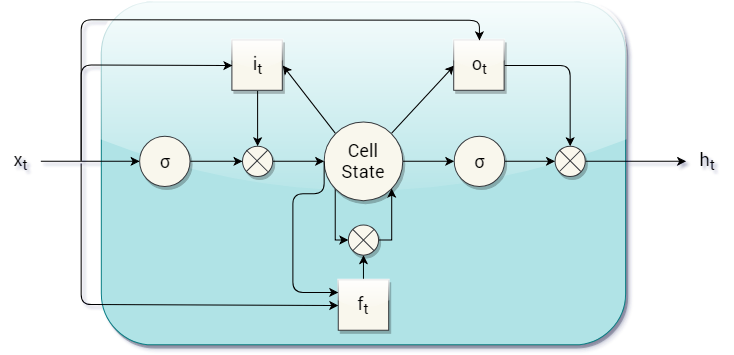
\includegraphics[width=0.6\linewidth]{graphics/lstm/lstm_peephole.png}
	\caption{
		Peephole LSTM module variation.
	}
	\label{fig:lstm_peephole}
\end{marginfigure}

\subsection{Convolutional LSTM}
Another variation of LSTM first proposed by \citet{Shi:2015:CLN:2969239.2969329}, which used the LSTM's long-term dependency property in conjunction with a Convolutional Neural Network in order to process multiple subsequent image frames and retain contextual knowledge of different scenes. Figure~\ref{fig:lstm_conv} demonstrates the operation of Convolutional LSTMs.

The operations which take place are the following:

\begin{itemize}
	\item {$h_{t}$} - The hidden gate, denoted by {$o_{t} \circ \sigma_{h}(c_{t})$}
	\item {$c_{t}$} - The current cell state, denoted by {$f_{t} \circ c_{t-1} + i_{t} \circ \sigma_{c}(W_{c} {\displaystyle *} x_{t} + U_{c} {\displaystyle *} h_{t-1} + b_{c})$}
	\item {$o_{t}$} - The output gate, denoted by {$\sigma_{g}(W_{o} {\displaystyle *} x_{t} + U_{o} {\displaystyle *} h_{t-1} + V_{o} \circ c_{t-1}+ b_{o})$}
	\item {$i_{t}$} - The input gate, denoted by {$\sigma_{g}(W_{i} {\displaystyle *} x_{t} + U_{i} {\displaystyle *} h_{t-1} + V_{i} \circ c_{t-1}+ b_{i})$}
	\item {$f_{t}$} - The forget gate, denoted by {$\sigma_{g}(W_{f} {\displaystyle *} x_{t} + U_{f} {\displaystyle *} h_{t-1} + V_{f} \circ c_{t-1}+ b_{f})$}
\end{itemize}

\begin{marginfigure}
	\centering
	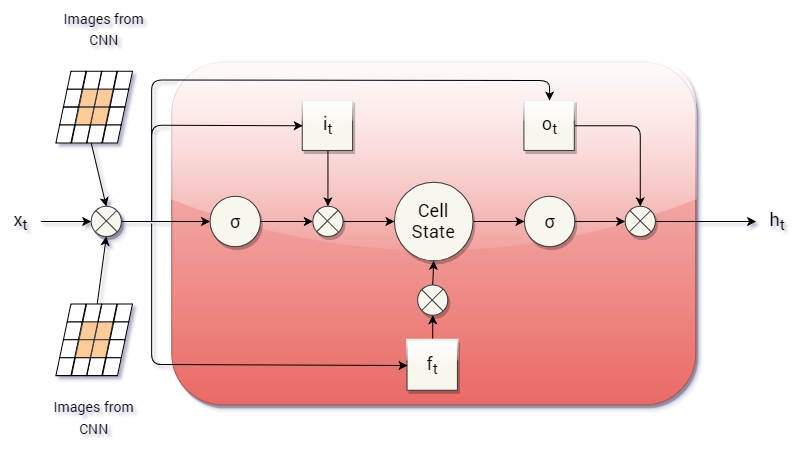
\includegraphics[width=0.6\linewidth]{graphics/lstm/lstm_conv.png}
	\caption{
		Peephole Convolutional LSTM module variation.
	}
	\label{fig:lstm_conv}
\end{marginfigure}

\subsection{Gated Recurrent Units (GRU)}
This variation, first proposed by \citet{cho-al-emnlp14}, is very similar to the LSTM architecture in that it also a gated network, depicted in Figure~\ref{fig:gru}. The main architecture of a GRU consists of a fully gated unit, where for time {$t = 0$} and output {$y_{t} = 0$}, the output vector {$h_{t}$} is defined as:

\begin{equation} \label{GRU transfer function}
	h_{t} = z_{t} \circ h_{t-1} + (1-z_{t}) \circ  (W_{h}x_{t} + U_{h}(r_{t} \circ h_{t-1}) + b_{h})
\end{equation}

where

\begin{itemize}
	\item {$x_{t}$} is the input gate
	\item {$z_{t}$} is the update gate, denoted by the function {$\sigma_{g}(W_{z}x_{t} + U_{z}h_{t-1} + b_{z})$}
	\item {$r_{t}$} is the reset gate, denoted by the function {$\sigma_{g}(W_{r}x_{t} + U_{r}h_{t-1} + b_{r})$}
\end{itemize}

\begin{marginfigure}
\centering
	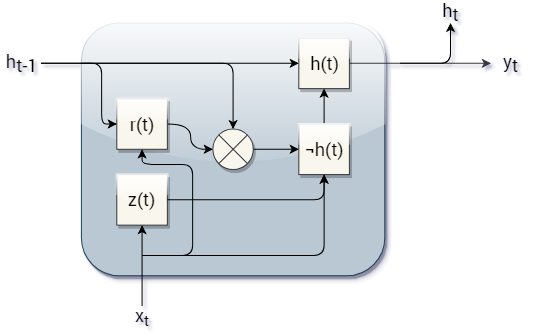
\includegraphics[width=0.6\linewidth]{graphics/lstm/gru.png}
	\caption{
		Structure of GRU, based on figure by \citet{gruthithuhuong2016}.
	}
	\label{fig:gru}
\end{marginfigure}

In conclusion, LSTMs are an excellent deep learning tool for time-series problems such as Natural Language Processing, where sentence fragments require memory \citep{Graves:2006:CTC:1143844.1143891,Gers:2001:LRN:2325782.2326800,Schmidhuber:2005:EHN:1642293.1642430,Schafer:2006:LLT:2125268.2125278}. However, those are not the only applications of LSTMs. Other applications can involve speech recognition \citep{Saon:2017:RAC:3266800.3266802}, handwriting recognition \citep{Graves:2009:NCS:1525650.1525782}, patient subtyping \citep{Baytas:2017:PSV:3097983.3097997}, and many more applications. Handling context is very important in many domains, and as such, LSTMs have been and will continue to be used and improved on to support the ever-growing problems in Machine Learning.

\index{lstm|)}